\clearpage
\section{The mechanism analysis in full}
\label{app:mechanism}

This appendix expands the mechanism paragraph of \S\ref{sec:discussion}.

\subsection{The faithfulness statistic}
\label{app:faithfulness}

\begin{figure*}[t]
\centering
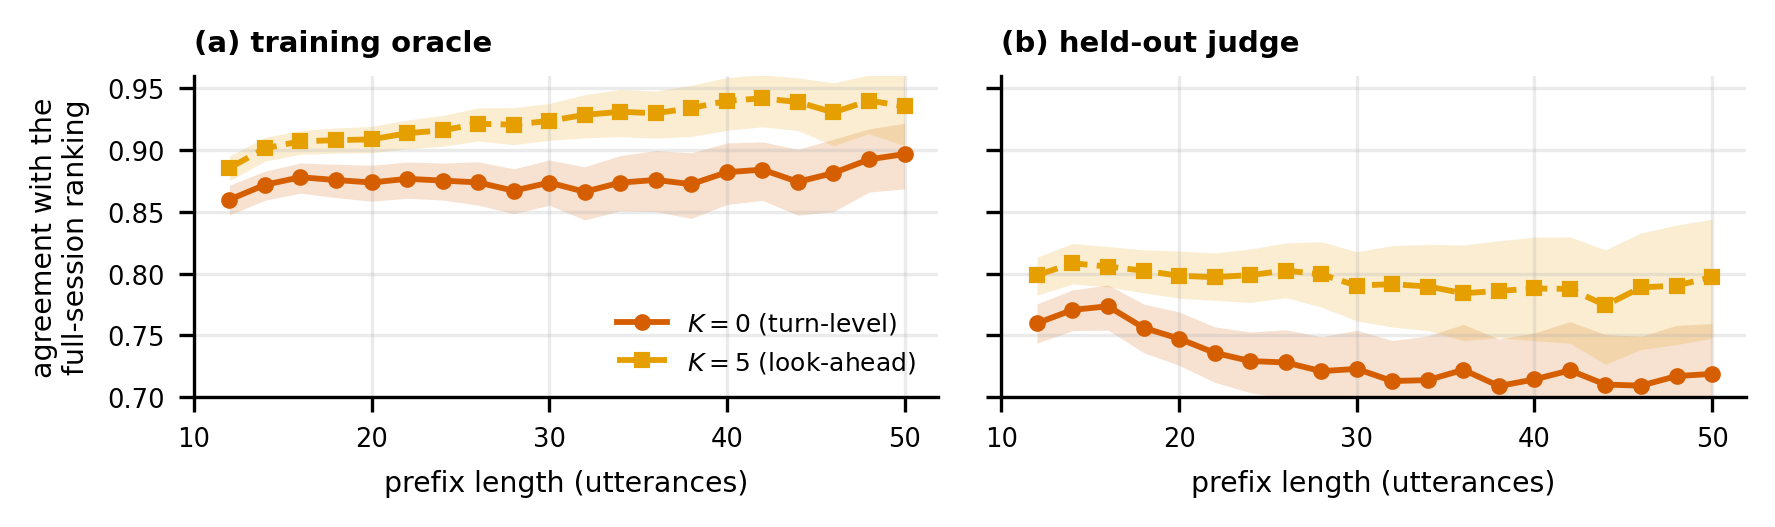
\includegraphics[width=0.94\textwidth]{figures/faithfulness_grpo.png}
\caption{Faithfulness of the training reward by prefix length, iterations 1--10 pooled, under
\textbf{(a)} the training oracle and \textbf{(b)} the held-out judge: the share of candidate pairs,
compared within one (run, iteration, conversation-length) cell, that the training reward orders the
way the full-session score does. Chance is $0.5$; bands are conversation-level cluster-bootstrap
intervals. The value at the shortest admitted prefix, 12 utterances, is the $86$--$89\%$ figure of
\S\ref{sec:lagrpo}.}
\label{fig:faithfulness}
\end{figure*}

The training reward scores a \emph{partial} conversation; the evaluation scores the whole session.
The gap between them is measurable as pairwise rank agreement: among candidate turns compared
within one (run, iteration, conversation-length) cell, how often does the training reward order
them the way the full-session score eventually does? Chance is $0.5$; intervals are
conversation-level cluster bootstraps.

Pooled over the ten iterations, agreement is $0.909$ $[0.900, 0.917]$ under $\Kf$ against $0.873$
$[0.861, 0.884]$ under $\Kz$ on the training oracle, and $0.800$ against $0.747$ on the held-out
judge; both differences have intervals excluding zero, and $\Kf$ is the more faithful run at 7 of
10 iterations under both judges. By prefix length, agreement at the shortest admitted prefix (12
utterances) is $0.860$ under $\Kz$ and $0.886$ under $\Kf$ on the training oracle, and it does
not fall with length ($0.897$ and $0.936$ at 50 utterances); this is the $86$--$89\%$ figure
quoted in \S\ref{sec:lagrpo} (Figure~\ref{fig:faithfulness}). Because MCL${=}12$ admits no shorter prefix, this experiment cannot
itself reproduce the pilot's short-prefix finding; it shows that the knob operates above it. Two qualifications travel with that number. First, the
iteration-level Wilcoxon test, with the ten iterations rather than the branch pairs as the unit of
observation, does \emph{not} clear $.05$ ($p = .084$ training oracle, $p = .193$ held out). The
pooled interval treats branch pairs as independent and is the more permissive of the two, so we
describe the difference as small and consistent rather than significant. Second, at iteration $n$
the two runs are \emph{different policies} generating \emph{different conversations}, so this
comparison measures a joint property of the scoring rule and of the trajectory the scoring rule put
the policy on; it cannot separate them.

\subsection{At a matched policy, the effect disappears}

There is exactly one cut in this design where the scoring rule is close to the only difference: the
first iteration, where both runs start from the same Base policy and differ only in whether five
simulated turns were appended before the oracle saw each candidate. At that cut nothing is
detectable. Both deltas straddle zero ($\Kf - \Kz$ agreement, training oracle: $-0.015$
$[-0.059, 0.026]$; held-out judge: $+0.014$ $[-0.048, 0.075]$), and the per-length-bin breakdown
points in opposite directions on the two judges: 17 of 20 bins favour $\Kz$ under the training
oracle, 17 of 20 favour $\Kf$ under the held-out judge. An effect whose sign depends on the judge
is not distinguishable from zero. The matched-policy cut is also the weakest-powered one (a single
model state per run, and only approximately matched, since the policy drifts within the iteration
under $K$-specific rewards), so this is an absence of evidence rather than evidence of absence; we
report it alongside the pooled estimate.

\subsection{Dispersion, and the iteration-10 inversion}

The mean best-minus-worst margin within a group is $1.300\times$ larger under $\Kf$
$[1.275, 1.326]$; the within-group standard deviation grows by $1.293\times$ $[1.267, 1.317]$; the
ratio of the two is $1.006$ $[1.002, 1.010]$, a pure rescaling that the advantage normalisation
absorbs.

One iteration inverts the \emph{level} of this. At training iteration 10 the margin ratio drops to
$0.679$: $\Kf$'s within-group margins are smaller than $\Kz$'s there. Both sides move. $\Kz$'s mean
margin jumps from $0.248$ to $0.339$ while $\Kf$'s falls from $0.268$ to $0.230$. The $\Kz$ jump
coincides with the iteration in which its over-praise rate jumps (the keyword marker goes
from $0.094$ to $0.671$ between iterations 9 and 10), which is what a group containing both
over-praising and non-over-praising candidates would do under a judge that rewards praise: the
pool splits and the best--worst gap widens. The $\Kf$ decline is the mirror image, a converging policy
whose eight samples the oracle scores increasingly alike. This does not break the rescaling result:
at that same iteration the ratio of ratios is $0.964$, so margin and standard deviation still move
together. We offer the over-praise account as consistent with the timing, not as demonstrated.

\subsection{What the training reward pays for praise}
\label{app:premium}

\begin{figure}[t]
\centering

\includegraphics[width=0.48\textwidth]{figures/praise_premium_grpo.png}
\caption{\textbf{(a)} The training reward's premium for praise: in each group of eight candidates
that holds both a reply containing a keyword-marker phrase and one without, the mean
within-group reward z-score of the praising replies minus that of the others, averaged over such
groups ($\pm 1.96$ SE), by the iteration of the model the candidates were sampled from.
\textbf{(b)} The share of groups that hold both kinds.}
\label{fig:premium}
\end{figure}

The keyword marker (Appendix~\ref{app:marker}) lets us ask whether the training reward itself pays
for praise, separately from how often the policy praises (Figure~\ref{fig:premium}). Within each
group of eight candidates we z-score the rewards, and in the groups that hold both a praising reply
and a non-praising one we take the praising replies' mean z minus the others'. Early in training
such groups are rare (about $2\%$ of groups, panel b) and the premium is noisy, negative under
$\Kz$ at iterations 0--1 and under $\Kf$ at iteration 2. From iteration 4 both rewards pay for praise: $0.22$--$0.33$
within-group SD under $\Kz$ over iterations 4--7 ($z \geq 2.8$ at each) and $0.16$--$0.21$ under
$\Kf$ ($z$ above 2 only at iterations 6--7). Both dip at iteration 8; at iteration 9 the $\Kz$
reward still pays $0.16$ ($z = 5.7$) and the $\Kf$ reward $0.04$ ($z = 1.1$). The share of groups
holding both kinds rises under both runs, and faster under $\Kz$: from iteration 7 on it is about
half of $\Kz$'s groups, against $0.28$--$0.44$ of $\Kf$'s.

\subsection{The update-direction proxy}

Writing each iteration's update direction as the advantage-weighted sum of its candidates' sentence
embeddings, $\operatorname{normalise}(\sum_g w_g \cdot \mathrm{emb}(t_g))$ with $w_g$ the
standardised group-relative advantage that scales each completion's gradient, the two runs' pooled
directions have a cosine of $0.804$, or $0.851$ once divided by the attenuation ceiling ($0.945$)
that two split-half-noisy estimates can reach at all. This is an embedding-space proxy, not the
gradient: it measures the semantic direction of what the update prefers, and it says the $\Kz$ and
$\Kf$ policies are pushed along substantially the same direction.
